\documentclass[11pt]{amsbook}

\usepackage{../HBSuerDemir}	% ------------------------
\usepackage{graphicx}
\usepackage{wrapfig}

\begin{document}

% ++++++++++++++++++++++++++++++++++++++
\hPage{b1p1/23}
% ++++++++++++++++++++++++++++++++++++++


% =======================================

%Venn Diagram-(with wrapfig)-------------------------------
\begin{wrapfigure}[3]{r}{0.25\textwidth}
	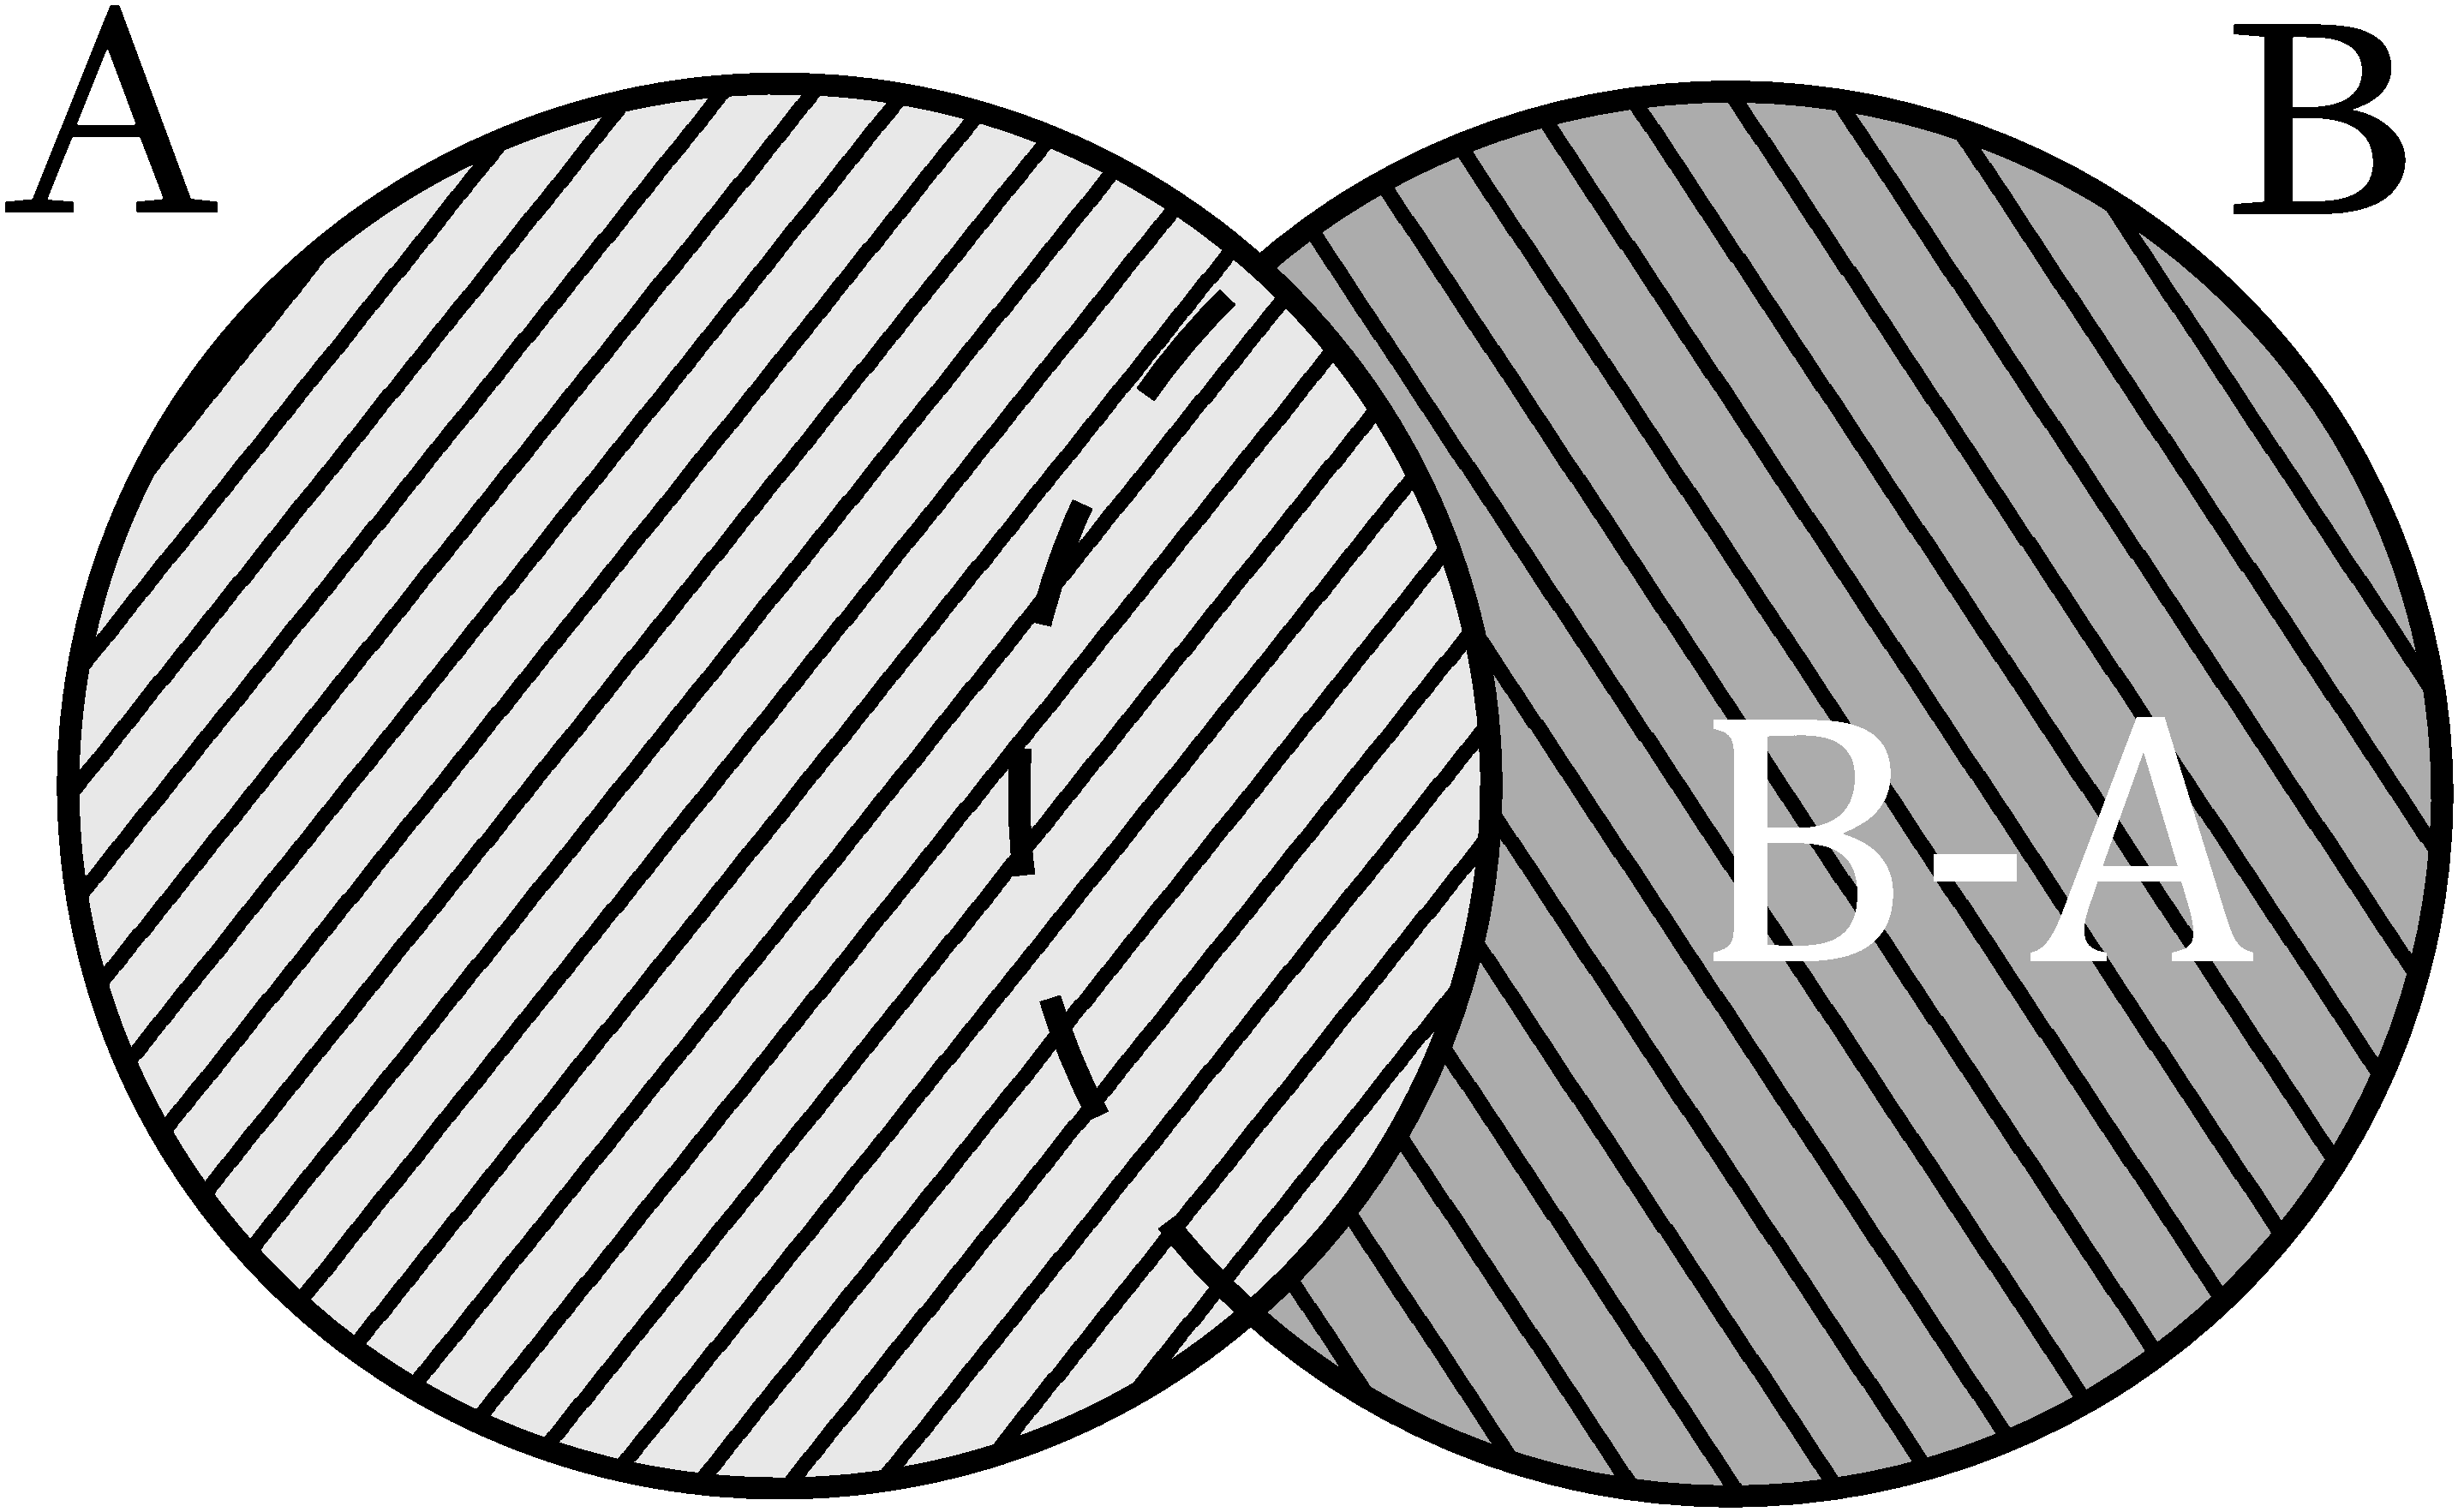
\includegraphics[width = 0.25\textwidth, keepaspectratio = true]{images/b1p1-023-fig01}
\end{wrapfigure}

%----------------------------------------------------------------
Examining the accompanying Venn diagram\footnote{image alignment requires wrapfig package} one immediately gets the relationships 

\begin{align*}
	n(A \cup B) &= n(A) + n(B-A)\\
	n(B-A) &= n(B) - n(A \cap B)\\
\end{align*}

\noindent which when added member to member give

\begin{equation*}
	n(A \cup B) = n(A) + n(B) - n(A \cap B)
\end{equation*}

% =======================================
\subsection{Complement}
	When $A \subseteq S$, the difference $S - A$ is called the \hDefined{complement} of $A$ with 
	respect to (w.r. to) the set $S$, and denoted by

\begin{equation*}
	\complement_{S} A \textrm{\quad\quad (Read: The complement of $A$ w.r. to $S$)}
\end{equation*}

If $S$ is taken as a universal set $U$, the notation for the complement of
$A$ is simply $A'$. The immediate corollaries are clear:

\begin{equation*}
	(A')' = A, \quad\quad U' = \emptyset, \quad\quad \emptyset' = U
\end{equation*}

\begin{exmp}
	For $S = \{2, 4, 5, 6, 9\}$ and $A = \{2, 6, 9\} \subseteq S$ find the complement of $A$ w.r. to $S$.\\
	\begin{equation*}
		\complement_{S} A = S - A = \{4, 5\}
	\end{equation*}
\end{exmp}

\begin{exmp}
	$\complement_{R} \hSoQ = \hSoQ'$
\end{exmp}

\begin{exmp}
	Verify the following relations by the use of Venn diagrams
\end{exmp}

% =======================================================
\end{document}  